\section{Introduction}
\label{sec:intro}


%\begin{figure}[t]
%	\centering
%	%	\vspace{-3mm}
%	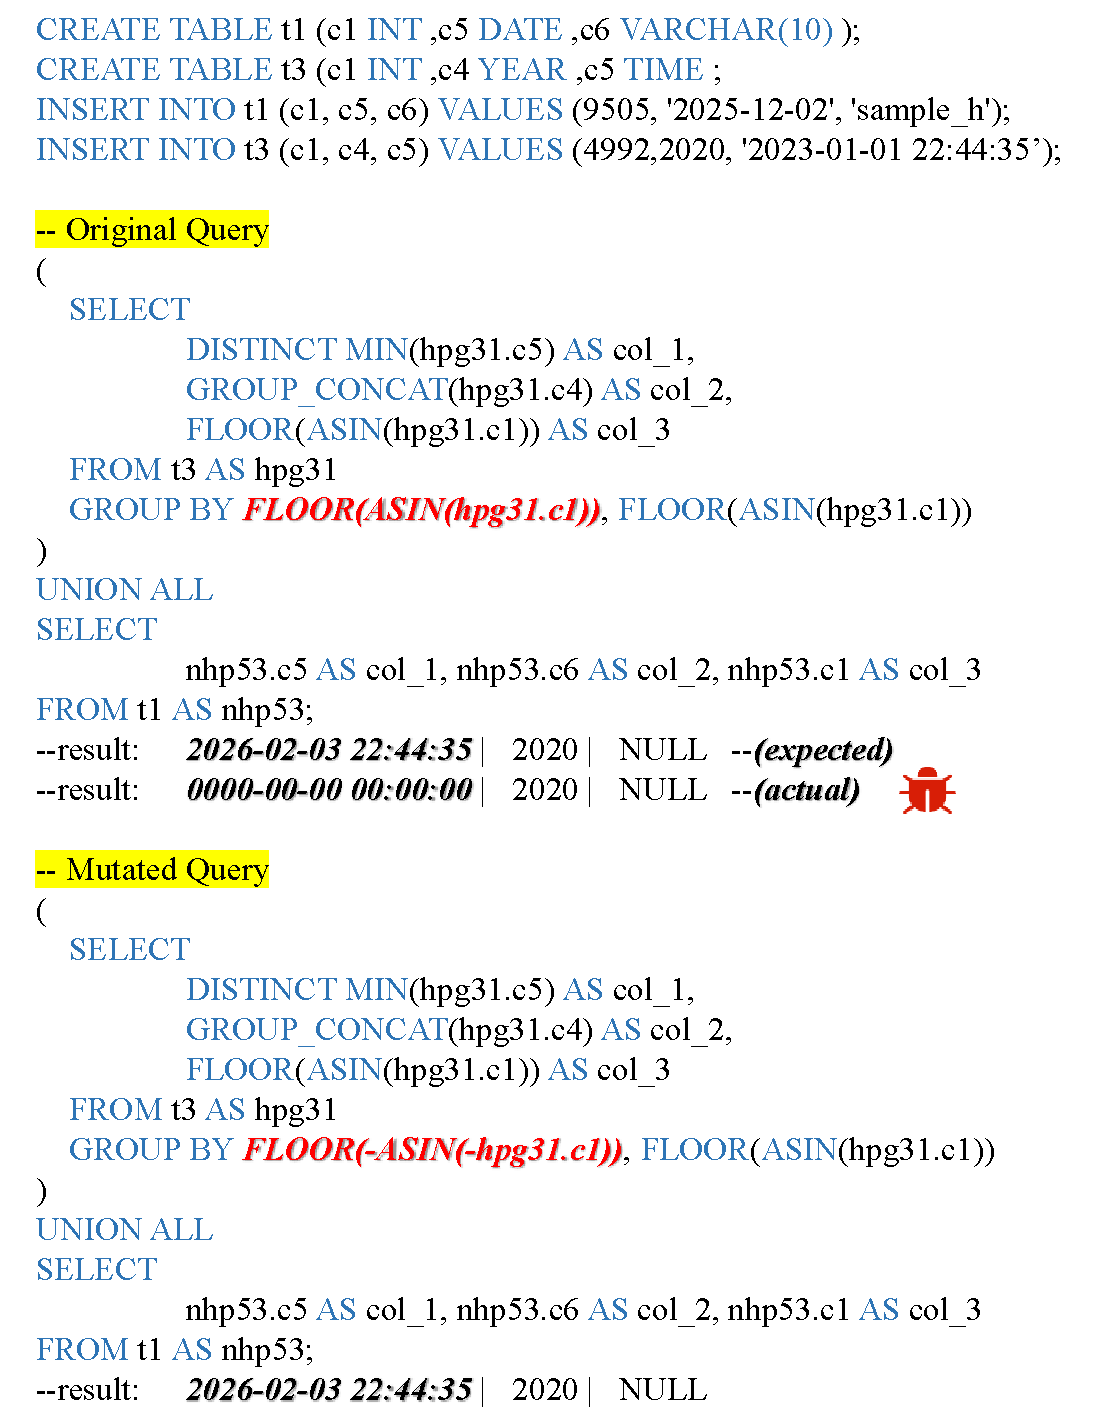
\includegraphics[width=1\linewidth]{./images/motivating_example.pdf} 
%	\vspace{-6mm}
%	\caption{\textbf{Queries exposing a logical bug in a built-in SQL function in Percona Server.}}
%	\label{fig:motivating example}
%	\vspace{-5mm}
%\end{figure}


% Contribution
%Overall, we make the following contributions:
%\begin{itemize}[leftmargin=10pt]
%	\item We propose a novel methodology \textit{Function Property--Driven Metamorphic Testing} for systematically detecting logical bugs in built-in SQL functions.
%	\item We implement \toolname\ as a DBMS testing tool, which automatically generates, mutates, and verifies SQL queries based on \textit{Function Property--Driven Metamorphic Testing}, enabling the detection of logical bugs in SQL functions.
%	\item We evaluate \toolname\ on six real-world DBMSs and find \reported\ previously unknown logical bugs.  
%	To further facilitate research on DBMS testing, we open-source \toolname\ at \url{https://anonymous.4open.science/status/FPMT-DBTesting-D3CA}.
%\end{itemize}






